\chapter{An Analysis of the Development of the Rhythm of English-L2 by Brazilian Learners through Rhythmic Metrics and Acoustic Parameters}\label{ch:leonardoanton9}
\chapterauthor[1]{Leonardo Antonio Silva Teixeira}
\chapterauthor[1]{Ronaldo Mangueira Lima Jr.}
\begin{affils}
\chapteraffil[1]{Universidade Federal do Ceará}
\end{affils}

\begin{abstract}
The aim of this study is to describe and discuss the development of L2 English
rhythm by Brazilian learners through rhythmic metrics and prosodic-acoustic
parameters that characterize the oral production of these learners at different
stages of L2 development. Five Brazilian learners of English-L2 were recorded
reading a text in English at the beginning of their college studies in English
Language Teaching, and again four semesters later, after having taken two
English phonology courses. They were also recorded reading a version of the
text translated into Portuguese. Besides the learners, five native speakers of
North American English were recorded reading the same text in English. Data
were manually segmented into vowel units (V), consonant (C), vowel-vowel (VV),
sentences (S) and higher prosodic units - chunks (CH) in PRAAT \citep{boersma_praat},
and the parameters were automatically by means of a script.
Data were statistically treated via R \citep{r2021} %(R CORE TEAM, 2021) 
through the implementation of mixed-effects regression models. Results placed Brazilian
Portuguese and English-L1 in different rhythmic spaces, as predicted by the
literature; in the durational dimension, the metrics positioned the English-L2
of the first recording far from both English-L1 and Brazilian Portuguese; in
the f0 and intensity dimensions, however, the acoustic parameters placed the
English-L2 of the first recording closer to Brazilian Portuguese. In both
dimensions, the English-L2 of the subsequent recording was closer to
English-L1, suggesting a developmental route towards the target language. The
results also suggest positive effects of the explicit teaching of
pronunciation.
\end{abstract}



%%%%%%%%%%%%%%%%%%%%%%%%%%%%%%%%%%%%%%%%%%%%%%%%%%%%%%%%%%%%%%%%%%%%%%
\section{Introduction}
Regarding research in non-native language (L2) development, there seems to be
greater emphasis on segmental aspects rather than prosodic ones \citep{li2014,thomson2015}.
This tendency is also reflected in L2
acquisition models \citep{flege2021,best2007}, 
which emphasize segmental aspects, providing little support to the understanding of L2 prosodic
development. 
%There is also evidence that rhythm can influence the communication
%process in a global way, affecting degrees of perceived foreign accent and
%intelligibility \citep{silva2020}.
Among prosodic features, rhythm is the least explored \citep{cumming2010,gut2012,whitworth_speech_2002},
despite evidence that demonstrates it can influence the communication process in a global way, 
affecting degrees of perceived foreign accent and intelligibility \citep{silva2020}.

The scarcity of studies on the acquisition of L2 rhythm may be related to the
difficulty of establishing the physical reality of such construct. There are at
least three trends on research regarding linguistic rhythm. Lloyd James (1940),
as cited in \citet{abercrombie1971}, relied on the dichotomy Morse code versus
machine gun to illustrate the perceptual difference between English and
Spanish, respectively. \citet{pike1945} formalized that difference by proposing a
rhythmic approach based on the type of units that stood up in such languages:
stress-timed languages, for which interstress intervals would be the most
prominent units, and syllable-timed languages, for which syllables would be
such units. Later, \citet{abercrombie1971} proposed that those rhythmic units would
be isochronous, that is, of the same duration. However, the isochrony paradigm
proved to be empirically unsustainable since intervals of the same duration are
not found in the acoustic signal \citep{cumming2010}.

From the mid-90s, a second trend of studies in linguistic rhythm emerges, in
which the rhythmic patterns are investigated by means of the durational
characteristics of the reference intervals (vowels, consonants, syllables,
etc.), which can be computed by statistical indexes called rhythmic metrics.
\citet{ramus1999} proposed the standard deviation of the duration
of consonantal intervals (ΔC) and the percentual of the total duration of the
utterance composed of vowel intervals (\%V). Those metrics were able to
spatially discriminate languages considered syllable-timed (French, Spanish,
Italian and Catalan), stress-timed (English, Polish and Dutch) and mora-timed
languages (Japanese) \citep{ladefoged1975} on a plane with ΔC and \%V on each axis.%,
%as can be seen in Figure \ref{leo-fig01}, reproduced from the original paper:

%\begin{figure}
%\centering
%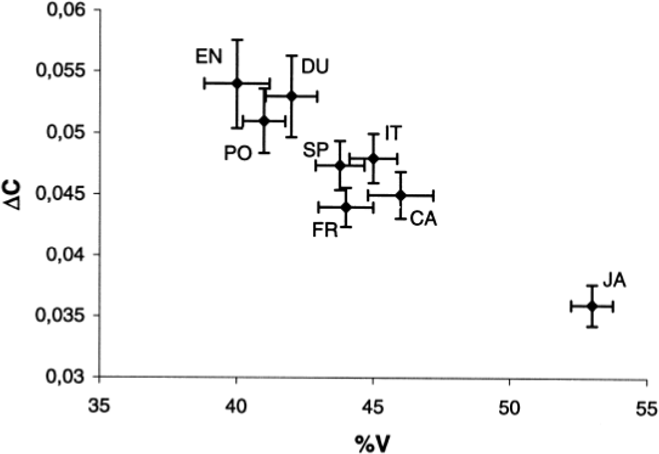
\includegraphics[width=0.9\linewidth]{imgs/leo-fig01.png}
%\caption{Distribution of languages over the (\%V, ∆C) plane. Error bars
%represent 1 standard error. Source: \citet[p.~273]{ramus1999}.}
%\label{leo-fig01}
%\end{figure}

The present study follows a third trend on research on linguistic rhythm, which
defines it as a function of the distribution of prominent elements in the
acoustic signal, which involves several acoustic dimensions – duration,
fundamental frequency (f0) and intensity, and may be influenced by the native
language of the speaker \citep{cumming2010,fuchs2016,silva2020}.
Thus, this study was guided by the following questions: (i) how do the metrics
and acoustic parameters place North American English-L1, Brazilian English-L2,
and Brazilian Portuguese (BP)-L1 in the rhythmic space? (ii) What is the
influence of the rhythm of BP-L1 on the development of English-L2 of learners?
(iii) What is the effect of explicit pronunciation teaching on learners'
English-L2 rhythm development? The following hypotheses were raised: (i) PB-L1,
English-L1 and English-L2 are rhythmically different systems; (ii) there will
be rhythmic differences between the English-L2 of the speakers in the two
different stages of development whose recordings were analyzed; (iii) the
English-L2 of the first recording should be more dissimilar to English-L1 due
to L1 transfer and lack of explicit instruction. 

%%%%%%%%%%%%%%%%%%%%%%%%%%%%%%%%%%%%%%%%%%%%%%%%%%%%%%%%%%%%%%%%%%%%%%%
\section{Methods}
As for the participants, the experimental group was composed of five BP-L1
speakers, who were also learners of English-L2. They were all college students
of English Language Teaching, being four men and one woman, aged between 18 to
24. The control group comprised five English-L1 speakers, all Canadians, being
one man and four women, aged 23-34. Four corpora of oral production were
analyzed in this study: English-L1, PB-L1, English-L2 (1) and English-L2 (4).
The data of English-L2 were obtained by means of recordings of the Brazilian
learners reading the first paragraph of a text in two different moments, before
and after completing courses in English Phonetics and Phonology. Those were the
first and fourth recording made so they are referred to as English-L2 (1) and
English-L2 (4). The data of English-L1 resulted from the reading of the same
text by the control group. Finally, the Portuguese-L1 data came from the
reading of the Portuguese version of the text by the Brazilian learners. The
recordings took place in a silent room with a cardioid Shure MX150B lapel
microphone connected to a Zoom 4HnSP recorder. The audio was captured in mono,
with a sampling rate of 44.1 kHz, and saved in wav format.


Data were manually segmented into vowel units (V), consonant (C), vowel-vowel
(VV), that is, the interval between the acoustic onset of a vowel and the onset
of the adjacent one, sentences (S) and higher prosodic units - chunks (CH) in
PRAAT \citep{boersma_praat}, and the script Metrics \& Acoustics Extractor
\citep{silva2020} was used to extract the parameters. Following \citet{silva2020},
the term metric(s) is used in this research to refer
to the duration-based parameters, and the term acoustic parameter(s) refers to
the f0, speech rate and intensive-related ones. The table below presents a
summary of the metrics and acoustic parameters analyzed in this study and the
types of segments they compute:

%%TABLE
\begin{table}
\caption{Rhythm metrics and prosodic-acoustic parameters analyzed in this study}\label{leo-tab01}
\begin{scriptsize}
\begin{tabular}{@{}p{3.1cm}p{1.6cm}p{2cm}p{1.5cm}@{}}
\toprule
\multicolumn{2}{c}{METRICS\protect\footnotemark[1]} & \multicolumn{2}{c}{ACOUSTIC PAREMETERS}\\
Parameters & Segment of application & Parameters & Segment of application \\
\midrule 
Percentual (\%) & V, C & f0 median & S, CH \\
Standard-deviation (∆) & V,C (V ou C), VV & f0 peak & S, CH \\
Variation coefficient (Varco)\protect\footnotemark[2] & V,C (V ou C), VV &  f0 minimum & S, CH \\
Raw pairwise variability index (r-PVI)\protect\footnotemark[3] & V,C (V ou C), VV & f0 standard deviation & S, CH \\
Normalized pairwise variability index (n-PVI)\protect\footnotemark[4] & V,C (V ou C), VV & f0 skewness & S, CH \\
Rhythm ratio (RR)\protect\footnotemark[5] & V,C (V ou C), VV & Mean of f0 first derivative (μΔ1- f0) & S, CH \\
Variability index (VI)\protect\footnotemark[6] & V,C (V ou C), VV & Standard deviation of f0 first derivative (σΔ1- f0) & S, CH \\
\multirow{6}{=}{Yet another rhythm determination (z-score duration) (YARD)\protect\footnotemark[7]} & \multirow{6}{*}{V,C (V ou C), VV} & Skewness of f0 first derivative (skΔ1- f0) & \\
   &  & Speech rate (SR) & VV, S, CH \\
   &  & f0 rate (f0-R)  & S, CH \\
   &  & Spectral emphasis & S, CH \\
   &  & Mean of normalized syllable-peak duration (μdur- Sil) & VV, S, CH \\
   &  & Mean duration of pauses (μdur-\#) & S, CH \\
\bottomrule
\end{tabular}
\end{scriptsize}
\end{table}
\footnotetext[1]{See \citet{fuchs2016} for a comprehensive account of rhythmic metrics.}
\footnotetext[2]{Standard deviation of the segment duration divided by the mean, multiplied by 100.}
\footnotetext[3]{Mean of the differences between successive segments.}
\footnotetext[4]{Mean of the differences between successive segments divided by their sum, multiplied by 100.}
\footnotetext[5]{Mean of pairwise quotients of adjacent segment durations, where the duration of the shorter is divided by the duration of the longer one and multiplied by 100.}
\footnotetext[6]{Mean of the differences between successive segments where the duration of each segment is normalised through division by the mean of all segments’ durations.}
\footnotetext[7]{Mean of the differences between successive segments where the durations are normalised by z-transformation.}

Data were then statistically treated via R \citep{r2021} %(R CORE TEAM, 2021) 
through the implementation of mixed-effects regression models, adopting language and
semester as predictor variables, and rhythmic metrics and acoustic parameters
as response variables.

%%%%%%%%%%%%%%%%%%%%%%%%%%%%%%%%%%%%%%%%%%%%%%%%%%%%%%%%%%%%%%%%%%%%%%%
\section{Results}
In this section, we present some of the significant results, based on the
mixed-effects regression models adjusted for each metric and acoustic
parameter, and the boxplots and bidimensional planes, in which the effect of
each corpus (independent variables) on the significant metrics and acoustic
measures (the dependent variables) can be visually inspected.

\subsection{Metrics}
Twenty out of the thirty employed metrics reached statistical significance for
at least two of the (inter) languages. One example of the mixed-regression
models that were implemented via R can be seen in Table \ref{leo-tab02}, which were adjusted
for the standard deviation of the duration of consonantal intervals (deltaC)
and the percentual of vocalic intervals (\%V).

\begin{table*}
\caption{Coefficients, confidence intervals (95\%) and p-Values for the two
linear mixed-effect regression models adjusted for ΔC and \%V. models: deltaC ~
Lang + (1|Chunk) + (1|Speaker) and percV ~ Lang + (1|Chunk) + (1 /
Speaker).}\label{leo-tab02}
\begin{small}
\begin{tabular}{@{}lllllll@{}}
\toprule
  & ΔC & \%V & & & & \\
Predictors & Estimates & CI & p & Estimates & CI & p \\
\midrule
(Intercept) & 46.48 & 36.17~--~56.79 & \textbf{\textless0.001} & 48.78 & 46.02~--~51.55 & \textbf{\textless0.001} \\
Lang {[}Eng-L1{]} & 21.94 & 7.35~--~36.52 & \textbf{0.004} & -9.66 & -12.97--~-6.35 & \textbf{\textless0.001} \\
Lang {[}Eng-L2 (1){]} & 58.71 & 44.13~--~73.30 & \textbf{\textless0.001} & -11.92 & -14.23~--~-9.61 & \textbf{\textless0.001} \\
Lang {[}Eng-L2 (4){]} & 37.61 & 23.02~--~52.19 & \textbf{\textless0.001}& -9.28 & -11.47~--~-7.09 & \textbf{\textless0.001} \\
\bottomrule
\end{tabular}
\end{small}
\end{table*}


Figure 2 shows the distribution of the 4 corpora over the planes formed by the
pairs ∆C-\%V and VarcoC-VarcoV in comparison to the data reviewed and obtained
by Arvaniti (2012). 

\begin{figure}
\centering
\subfloat[\label{leo-fig02-1}]{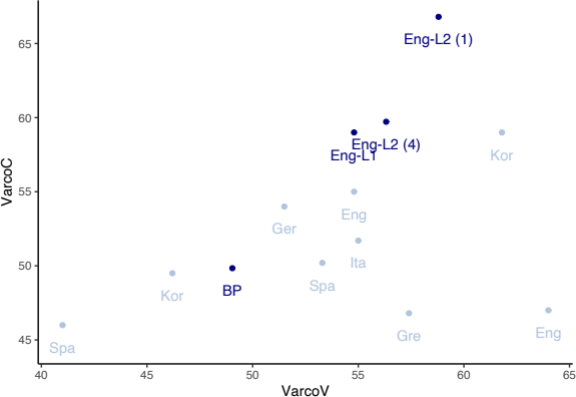
\includegraphics[width=0.7\textwidth]{imgs/leo-fig02.png}}\\
\subfloat[\label{leo-fig02-2}]{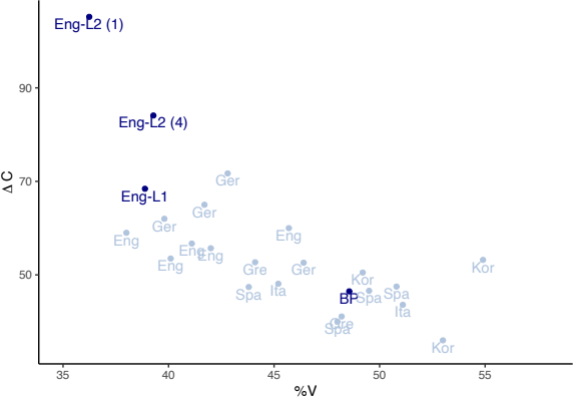
\includegraphics[width=0.7\textwidth]{imgs/leo-fig03.png}}\\
\caption{Present study data (dark blue) amid all the data reviewed and obtained
by Arvaniti (2012) (light blue) for ΔC - \%V (Figure \ref{leo-fig02} (a) and
VarcoC-VarcoV (Figure \ref{leo-fig02} (b)), in which Eng = English, Ger = German,
Gre = Greek, Spa = Spanish, UI = Italian, Kor = Korean. Source: Teixeira and Lima Jr. (2021).}
\label{leo-fig02}
\end{figure}


As can be seen in Figure \ref{leo-fig02} (a), English-L1 presented greater standard deviation
of consonantal intervals duration (ΔCEng-L1 = 68.41) compared to BP (ΔCBP =
46.48); and BP presented greater proportion of the utterance composed of vowel
intervals (\%VBP = 48.56) compared to English-L1 (\%VEng-L1 = 38,88). The data
of English-L2 (1) were positioned far from the two native languages, scoring ΔC
values quite high (ΔCEng-L2 (1) = 105.19) and the lowest proportion of vowel
segments (\%VEnglish-L2 (1) = 36.24). On the other hand, English-L2 (4) values
were much closer to English-L1 in relation to both axis (ΔCEngl-L2(4) = 84.08;
\%VEng-L2(4) = 39.28). As for VarcoC-VarcoV (Figure \ref{leo-fig02}),
English-L1, English-L2 (1), English-L2 (4) and BP were distributed analogously
to the plane ΔC-\%V, with the BP data recording the lowest values for both the
VarcoC (49.84) and VarcoV (49.04) axis, and English-L2 (1) presenting the
highest scores both in the VarcoC axis (66.8) and in relation to the VarcoV
axis (58.8). The fact that English-L2(1) assumed values far from the L1 (BP)
indicates no objective transference of durational prosodic patterns to the
learners’ interlanguages. On the other hand, the approximation between
English-L2(4) and English-L1 indicates a possible effect of explicit
instruction, among other factors, that may have influenced the temporal
(re)organization of the learners’ speech towards the prosodic patterns of the
target language. 

Regarding the data from Arvaniti (2012), BP grouped with languages considered
more syllable-timed, that is, with more durational regularity among the
segments of reference, such as Spanish and Italian. English-L1 results were
also consistent with the literature, gathering with the results for English and
German from other studies, which are considered languages with more
stress-timing tendency. 

The hierarchy of values for VarcoV-VarcoC and ΔC-\%V illustrates the dominant
positioning pattern for the significant metrics, as can be seen in Table \ref{leo-tab03}:
([+stress-timed] English-L2 (1) > English-L2 (4) > English-L1 > BP [+
syllable-timed]), except for \%V and RR, whose higher values indicate a
tendency towards syllable-timing.

\begin{table*}
\caption{Absolute means for the statistically significant metrics and standard
deviation (between parentheses) for BP, English-L1, English-L2 (1),
English-L2(1) and English-L2(4).\\$^\ast$ S stands for the phonetic syllable, which is the  vowel-vowel (VV) unit.}\label{leo-tab03}
\begin{small}
\begin{tabular}{@{}lllll@{}}
\toprule
Metric & BP & English-L1 & English-L2(1) & English-L2(4) \\
\midrule
\%V & 48.56 (3.16) & 38.88 (4.96) & 36.24 (5.36) & 46.48(8.02) \\
\%C & 51.44 (3,16) & 61.12 (4.96) & 63.76 (5.36) & 68.416(14.55) \\
∆V & 40.08 (10.81) & 41.16 (11.82) & 51.81 (12.79) & 105.192(32.6) \\
∆C & 46.48 (8.02) & 68.41 (14.55) & 105.192 (32.6) & 84.088(36.51) \\
∆S$^\ast$ & 133.4 (45.27) & 198.53 (77.44) & 217.46(97.65) & 184.75 (56.72) \\
VarcoV & 49.04 (8.49) & 54.80 (12.52) & 58.80 (11.30) & 56.32(14.81) \\
VarcoC & 49.84 (7,00) & 59 (11.89) & 66.80 (13.69) & 59.72(22.02) \\
rPVI-V & 65.1 (11.71) & 70.74 (14.84) & 96.98 (19.27) & 81.21(15.75) \\
rPVI-C & 48.22 (8.91) & 86.16 (20.23) & 116.84 (46.64) & 88.7(21.69) \\
rPVI-VC & 64.73 (18.72) & 83.58 (11.12) & 114.4 (38.18) & 89.1(14.53) \\
rPVI-S & 102.85 (40.24) & 130.66 (33.59) & 176.27 (90.03) & 137.96(44.62) \\
nPVI-C & 53.96 (7.21) & 68.56 (11.72) & 72.36 (12.14) & 64.84(11.46) \\
nPVI-VC & 59.76 (7.69) & 68.96 (11.09) & 72.6 (9.40) & 65.08(8.12) \\
RR-C & 61.17 (4.36) & 53.13 (6.29) & 50.97 (6.59) & 54.59(6.42) \\
RR-VC & 58.07 (4.35) & 52.8 (5.65) & 50.91 (4.97) & 54.55(4.59) \\
VI-V & 0.818 (0.166) & 0.981 (0.322) & 1.128 (0.302) & 0.894(0.188) \\
VI-V & 0.830 (0.037) & 0.924 (0.049) & 0.929 (0.052) & 0.934(0.059) \\
VI-VC & 0.684 (0.101) & 0.834 (0.157) & 0.859 (0.120) & 0.746(0.116) \\
VI-S & 0.516 (0.120) & 0.606 (0.136) & 0.615 (0.160) & 0.538(0.126) \\
YARD-VC & 0.717 (0.150) & 0.695 (0.133) & 0.869 (0.113) & 0.848(0.123) \\
\bottomrule
\end{tabular}
\end{small}
\end{table*}

%%%%%%%%%%%%%%%%%%%%%%%%%%%%%%%%%%%%%%%%%%%%%%%%%%%%%%%%%%%%%%%%%%%%%%
\subsection{Acoustic Parameters}
Five out of the twelve employed acoustic parameters reached statistical
significance: f0peak, σf0, σΔ1- f0, spectral emphasis (emph) and speech rate
(SR). 

As for the standard deviation of f0 (Figure 3.1), English-L1 presented the
highest standard deviation among the corpora analyzed (σf0Engl-L1 = 3.79),
followed by English-L2(4) (σf0Engl-L2(4) = 3.34), English-L2(1) (σf0Engl-L2(4)
= 2.71) and BP (σf0BP  = 2.62). The results for this parameter suggest a
gradual prosodic development of the learners towards the f0 variation patterns
of the target language. The standard deviation of f0 first derivative (σΔ1-f0)
(Figure 3.2) was also successful in the separation of the L1s and captured a
similar course of development to that found by σf0. The highest mean was scored
by English-L1(σΔ1- f0Eng-L1 = 5.51), the lowest mean was scored by BP (σΔ1-f0PB
= 3.61). The interlanguages registered intermediate values, but the mean
English-L2(4) was much closer to English-L1 (σΔ1-f0Eng-L2(1) = 3.73 <
σΔ1-f0Eng-L2(4) = 4.61).


\begin{figure}
\centering
\subfloat[\label{leo-fig03-1}]{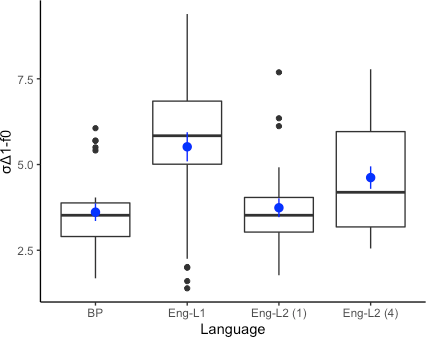
\includegraphics[width=0.7\textwidth]{imgs/leo-fig04.png}}\\
\subfloat[\label{leo-fig03-2}]{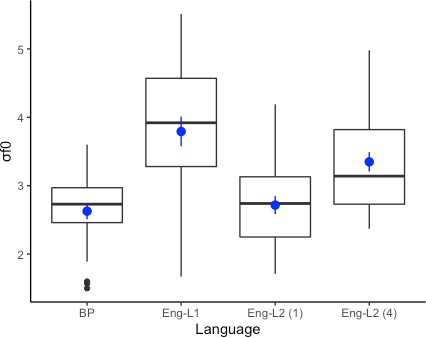
\includegraphics[width=0.7\textwidth]{imgs/leo-fig05.png}}\\
\caption{Boxplots of the means σf0 (Figure 3.1) and σΔ1- f0 (Figure 3.2 for
English-L1, English- L2(1), English-L2(4) and BP. The blue dots and lines
represent the means and standard errors respectively.}
\label{leo-fig03}
\end{figure}

The results for the f0 dimension must be interpreted with caution, since there
was an unbalance between male and female participants in both groups (control
group: 1 male, 4 female; experimental group: 4 males, 1 female). In fact, the
correlation between f0 and sex is evident when individual results are taken
into consideration. For instance, in the experimental group, it was observed
that participant N, the only female, is the one that had the highest f0 peak
(97.16), as well as the widest scopes of f0 (f0 peak minus f0 min) for BP
(17.18) and English-L2(4) (19.06). There was also a smaller variation between
the male learners f0 scope of English-L2(1) (A = 12.28; F = 15.68; K = 15.5; L
13.37) and English-L2(4) (A = 12.81; F = 15.09; K = 14.43; L = 15.1), in
comparison to the variation of the female participant, who went from 15.59 to
19.06 in the last recording. 

In the dimension of intensity, as visually demonstrated in Figure 4.1, spectral
emphasis was able to separate the L1s, with the highest mean for English-L1
among the analyzed corpora (emphEng-L1 = 4.34), which was higher than PB
(emphPB = 2.73). If we consider works that show the correlation between
spectral emphasis and phrasal stress \citep{heldner2001}, %(HELDNER, 2001) 
this result suggests that
native English speakers make more effort as an acoustic clue in stress marking
than Portuguese speakers. Regarding the interlanguages, English-L2 (1) obtained
the lowest mean of spectral emphasis, very close to BP values, (emphEng-L2(1) =
2.56), and English-L2 (4) got much closer to English-L1(emphEngl-L2 (4) =
3.23). This indicates L1 transfer at the intensity dimension, and a tendency
towards the prosodic patterns of English-L1 in the last recording.

\begin{figure}
\centering
\subfloat[\label{leo-fig04-1}]{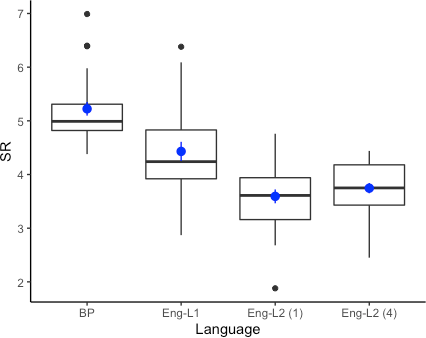
\includegraphics[width=0.7\textwidth]{imgs/leo-fig06.png}}\\
\subfloat[\label{leo-fig04-2}]{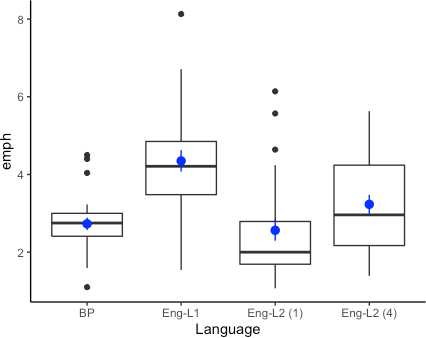
\includegraphics[width=0.7\textwidth]{imgs/leo-fig07.png}}\\
\caption{Boxplots of the means spectral emphasis (Figure \ref{leo-fig04} (a)) and speech rate
(Figure \ref{leo-fig04} (b)) for English-L1, English- L2(1), English-L2(4) and BP. The blue
dots and lines represent the means and standard errors respectively.}
\label{leo-fig04}
\end{figure}

As expected, the L1s presented higher speech rates, with BP registering a
higher mean compared to English-L1 (SRPB = 5.22 > SREngl-L1 = 4.43). In
addition, English-L2 (1) presented the lowest speech rate among the corpora
analyzed (SREngl-L2(1) = 3.59) and English-L2(4) registered a slightly higher
mean, closer to English-L1 (SREng-L2(4) = 3.74). The increase in the speech
rate of the interlanguages between the first and last recording may be related
to the effects of explicit instruction.

%%%%%%%%%%%%%%%%%%%%%%%%%%%%%%%%%%%%%%%%%%%%%%%%%%%%%%%%%%%%%%%%%%%%%%
\section{Discussion}
The metrics and parameters positioned BP, English-L1, English-L2 (1) and
English-L2 (4) as rhythmically different systems. There were differences
between the English-L2 of the speakers in the two different stages of
development and different developmental paths were captured as function of the
dimension of prominence.  This developmental path is consistent with the
definition of interlanguage that presents itself as a relatively independent
system of L1 and L2 \citep{li2014}, and with the non-linearity of the L2
development process \citep{lima2019}.

At the durational level, the dominant distribution pattern was ([+ stress-timed]
English-L2 (1) > English-L2 (4) > English-L1 > BP [+ syllable-timed]), with
English-L2(1) assuming the highest means among the four corpora, and
English-L2(4) getting closer values to English-L1. One possible explanation for
such behavior for English-L2(1) is that learners may have mobilized a process
of dissimilation of phonetic categories, displaying exaggerated durational
values to maintain the distinction between L1 and L2, similarly to what is
predicted by the Speech Learning Model for the segmental level \citep{flege1995,flege2021}. %(FLEGE, 1995,FLEGE; BOHN, 2021).

At the f0  dimension, the dominant distribution pattern ([+ f0 variability]
English-L1 > English-L2 (4) > English-L2 (1) > BP [- f0 variability]) placed
English-L1 with the highest means among the 4 corpora and BP with the lowest
means, which suggests English native speakers mobilize more complex and varied
f0 contours in speech. L1 transfer was more salient at the f0 level and seems
to be more persistent among men, which adds to \citet{urbani2012}. A tendency
towards the f0 prosodic patterns of the target language was also identified at
this level and could be an effect of explicit instruction. This effect may have
also influenced the greater speech rate ([+ speech rate] BP > English-L1 >
English-L2 (4) > English-L2 (1) [- speech rate]) and spectral emphasis ([+
spectral emph] English-L1 > English-L2 (4) > BP > English-L2 (1) [- spectral
emph]) for English-L2 (4), suggesting more fluency of the learners, and an
overall improvement in marking syllable stress, respectively.

%%%%%%%%%%%%%%%%%%%%%%%%%%%%%%%%%%%%%%%%%%%%%%%%%%%%%%%%%%%%%%%%%%%%%%
\section{Conclusion}
The metrics and acoustic parameters confirmed the first hypothesis that North
American English-L1, Brazilian English-L2, and BP-L1 are rhythmically
different systems. We confirmed the hypothesis that the data of English-L2 (1)
would be more dissimilar in relation to English-L1 compared to the data of
English-L2 (4), but orthogonal patterns of rhythmic development seem to coexist
as a function of the different dimensions of prominence. Nevertheless, the
approximation between the means of English-L2(4) and English-L1 in all
dimensions suggest positive effects of explicit pronunciation in the
development of prosodic features by learners of non-native languages.  As
future work, we intend to expand the analyzed corpora including the recordings
of the 2nd and 3rd semesters as well as the other paragraphs of the text, and
to analyze the correlation between the metrics and acoustic parameters and
perceived degrees of foreign accent, intelligibility, and comprehensibility.  



\section{Acknowledgment}

This study integrates a project that is partially financed by CNPq, process 438823/2018-4.

%%%%%%%%%%%%%%%%%%%%%%%%%%%%%%%%%%%%%%%%%%%%%%%%%%%%%%%%%%%%%%%%%%%%%%
\bibliographystyle{plainnat}
\bibliography{leonardoanton9.bib}


